\section{A-causal but BIBO Systems}
\begin{frame}
    \frametitle{Outline}
    \tableofcontents[currentsection]
\end{frame}

\begin{frame}
    \frametitle{A-causal but BIBO Systems}

    Recall that the polynomial $B^u(q^{-1})$ is Schur
    \pause

    $\,$

    The AR model $B^u(q^{-1}) y(k) = u(k)$ corresponds to the block diagram
    \begin{figure}
        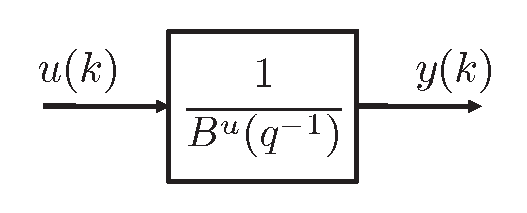
\includegraphics[width=4cm]{MVR_figs_ac1}
    \end{figure}
    \pause


    We can interpret the operator $\displaystyle{ \frac{1}{B^u(q^{-1})} }$ in two ways:
    \pause
    \begin{enumerate}
        \item
        Causal, but unstable
        \pause

        \item
        A-causal, but BIBO
    \end{enumerate}
\end{frame}

\begin{frame}
    \frametitle{Interpretation 1: Causal, but Unstable}

    We are considering the AR model $B^u(q^{-1}) y(k) = u(k)$ where
    \begin{align*}
        B^u(q^{-1}) = 1 + b_1^u q^{-1} + \cdots + b_{m_u}^u q^{-m_u}
    \end{align*}
    \paused
    \begin{align*}
        \longrightarrow \qquad (1 + b_1^u q^{-1} + \cdots + b_{m_u}^u q^{-m_u}) y(k) = u(k)
    \end{align*}
    \pause

    Interpreting the AR model as causal, but unstable corresponds to
    \begin{align*}
        y(k) & = u(k) - [b_1^u q^{-1} + \cdots + b_{m_u}^u q^{-m_u}] y(k) \\
        & = u(k) - b_1^u \, y(k-1) - \cdots - b_{m_u}^u \, y(k-m_u)
    \end{align*}
    \paused

    $\longrightarrow \qquad y(k)$ is a function of $u(k),u(k-1),u(k-2),\ldots$
\end{frame}

\begin{frame}
    \frametitle{Interpretation 2: A-causal, but BIBO}

    We are considering the AR model
    \begin{align*}
        (1 + b_1^u q^{-1} + \cdots + b_{m_u}^u q^{-m_u}) y(k) = u(k)
    \end{align*}
    \paused

    Interpreting the AR model as a-causal, but BIBO corresponds to
    \begin{align*}
        b_{m_u}^u q^{-m_u} y(k) & = u(k) - [1 + b_1^u q^{-1} + \cdots + b_{m_u-1}^u q^{-m_u+1}] y(k)
    \end{align*}
    \paused
    \begin{align*}
        \Rightarrow b_{m_u}^u y(k) & = q^{m_u} u(k) - [q^{m_u} + b_1^u q^{m_u-1} + \cdots + b_{m_u-1}^u q] y(k) \\
        \Rightarrow y(k) & = \frac{1}{b_{m_u}} [ u(k+m_u) - y(k+m_u) - b_1^u y(k+m_u-1) \\
        & \quad - \cdots - b_{m_u-1}^u y(k+1) ]
    \end{align*}
    \paused

    \alignbox{
        y(k) \textrm{ is a function of } u(k+m_u),u(k+m_u+1),u(k+m_u+2),\ldots
    }
\end{frame}

\begin{frame}
    \frametitle{A-causal but BIBO All-Pass Filter}

    Let $w(k)$ be the output of the a-causal, but BIBO ARMAX model
    \begin{align*}
        B^u(q^{-1}) w(k) = \bar{B}^u(q^{-1}) y(k)
    \end{align*}
    This corresponds to the block diagram
    \begin{figure}
        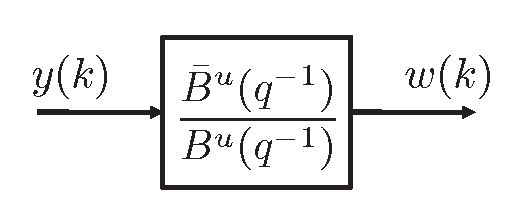
\includegraphics[width=4cm]{MVR_figs_ac2}
    \end{figure}
    \pause

    \textbf{Claim:}
    \begin{align*}
        \left| \frac{\bar{B}^u(e^{-j\omega})}{B^u(e^{-j\omega})} \right| = 1 \qquad \forall \omega \in [0,2\pi]
    \end{align*}
    \paused

    \textit{Proof:}
    \begin{gather*}
        \bar{B}^u(q) = q^{m_u} B^u(q^{-1}) \quad \Rightarrow \quad \bar{B}^u(q^{-1}) = q^{-m_u} B^u(q) \\
        \Rightarrow \quad | \bar{B}^u(e^{-j\omega}) | = | e^{-j\omega m_u} B^u(e^{j\omega}) | = | B^u(e^{j\omega}) |
            = | B^u(e^{-j\omega}) | \qquad \blacksquare
    \end{gather*}

\end{frame}

\begin{frame}
    \frametitle{A-causal but BIBO All-Pass Filter}

    \begin{figure}
        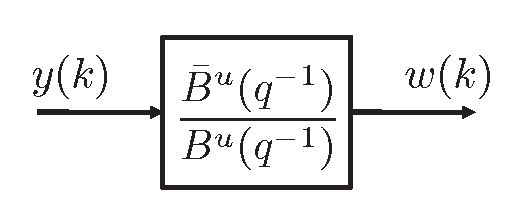
\includegraphics[width=4cm]{MVR_figs_ac2}
    \end{figure}

    The power spectral density of $w(k)$ is
    \begin{align*}
        \Phi_{WW}(\omega) = \left| \frac{\bar{B}^u(e^{-j\omega})}{B^u(e^{-j\omega})} \right|^2 \Phi_{YY}(\omega)
            = \Phi_{YY}(\omega)
    \end{align*}
    \pause

    Therefore
    \begin{align*}
        \Lambda_{WW}(0) = \frac{1}{2\pi} \int_{-\pi}^\pi \Phi_{WW}(\omega) d\omega
            = \frac{1}{2\pi} \int_{-\pi}^\pi \Phi_{YY}(\omega) d\omega
            = \Lambda_{YY}(0)
    \end{align*}
    \pause

    \alignbox{
        E\{w^2(k)\} = E\{y^2(k)\}
    }

\end{frame} 